\chapter{Lois de comportement}
\label{ch:ch5}

\section{Pourquoi en a-t-on besoin?}
La réponse en trois points :
\begin{enumerate}
	\item \textit{Décompte des équations et des inconnues} ; trop d'inconnues et pas assez d'équations.
	\item \textit{Liaison statique $\leftrightarrow$ cinématique} ; lier les forces aux déplacements.
	\item \textit{Nature du milieu continu} ; comportement différent en fonction du matériau.
\end{enumerate}
Ayant établi les équations pour tous les milieux continus, nous avons\footnote{$\tau$ est une 
	pression. La dérivée d'une pression par rapport à une composante spatiale donne bien une force par
volume, comme le reste des termes de cette équation.} :

\begin{center}
	\begin{tabular}{|c|c|c|c|}
		\hline
		\textbf{Equation}                       & \textbf{Nombre d'équations} & \textbf{Inconnues} & \textbf{Nombre 
		d'inconnues}\\
		\hline
		$\rho^\bullet + \rho\partial_i v_i = 0$ & 1                            & $\rho,v_i$         & 4              \\
		\hline
		$\begin{array}{ll}
		\rho v_i^\bullet &= f_i + \tau_{ij,j}\\
		\tau_{ij} &= \tau_{ji}
		\end{array}$                            & 3                            & $\tau_{(ij)}$      & 6              \\
		\hline
		                                        & 4 équations                 &                    & 10 inconnues   \\
		\hline
	\end{tabular}
	\captionof{table}{Récapitulatif}
\end{center}
Attention au décompte, les forces de volumes $f_i$ ne sont pas toujours connues : un gaz peut
avoir plusieurs quantités différentes de masse ! Mais comme $f_i = \rho F_i$ et que $F_i$ est
connu et que $\rho$ a déjà été compté, \textit{le compte est bon} si j'ose dire.\\

Dix inconnues pour quatre équations ? Problem? No ! Car le tenseur des contraintes, symétrique,
possède six composantes. Les composantes du tenseur permettent de lier les variables "cinématique" à des variables "statiques" :
\begin{itemize}
	\item $\tau_{ij}$ (contraintes) = fonction de $L_{ij}$ (déformations)
	\item $\tau_{ij}$ (contraintes) = fonction de $V_{ij}$ (vitesses de déformations)
\end{itemize}\ \\

On trouvera deux grandes catégories de lois de comportements : les fluides (dont les six composantes 
du vecteur de contraintes sont des fonctions des vitesses de déformations) et les solides (où 
les composantes sont fonction des déformations évanouissantes).

\section{Les fluides : les fluides parfaits et les fluides visqueux newtoniens}
\subsection{Le fluide parfait}
La loi de comportement du fluide parfait est : \\
\begin{wrapfigure}[2]{r}{3cm}
	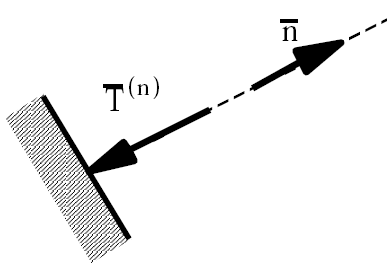
\includegraphics[scale=0.2]{ch5/image1.png}
	\captionof{figure}{Dessin pour $p > 0$}
\end{wrapfigure}
        
\prop{ \begin{equation}
	\tau_{ij} = -p\ \delta_{ij}
	\end{equation}
	où $p$ est la pression extérieure (voir schéma ci-contre pour le signe).\\
	On trouve alors : 
	\begin{equation}
		T^{(n)}_i = \tau_{ij}n_j = -pn_i\ \ \ \ \text{ou } \overline{T}^{(n)} = -p\overline{n}
	\end{equation}}\ \\
    
Ceci est valable pour toute direction ! En "déballant" $\tau_{ij}$, on s'aperçoit que le
fluide ne transmet que des contraintes normales et \textbf{jamais} de tangentielles ; le
cercle de Mohr se réduit à un point.
%\begin{equation}
%\tau_{ij} = \left|\begin{array}{ccc}
%-p & 0 & 0\\
% 0 & -p & 0\\
% 0 & 0 & -p
%\end{array}\right|
%\end{equation}
    
\begin{equation}
	\tau_{ij} =
	\begin{pmatrix}
		-p & 0  & 0  \\
		0  & -p & 0  \\
		0  & 0  & -p 
	\end{pmatrix}
\end{equation}

    
\subsection{Le fluide visqueux newtonien}
Pour ce "type" de fluide, on cherche à établir une loi de comportement de la forme 
\begin{equation}
	\tau_{ij} = f(V_{kl})
\end{equation}
où $f(V_{kl})$ est linéaire, c'est à dire tel que :
\begin{equation}
	\tau_{ij} = C_{ij} + D_{ijkl}V_{kl}
\end{equation}
Il s'agit d'un tenseur du $4^e$ ordre. On peut démontrer (admis) qu'un tel tenseur isotrope
peut s'exprimer en fonction de tenseurs isotropes du second ordre. Comme $C_{ij} = \alpha
\delta_{ij}$ on trouve:
\begin{equation}
	\begin{array}{ll}
		\tau_{ij} & = \alpha\delta_{ij} + \lambda \delta_{ij}\delta_{kl}V_{kl} + \beta                 
		\delta_{ik}\delta_{jl}V_{kl} + \beta' \delta_{il}\delta_{jk}V_{kl}  \\
		          & = \alpha\delta_{ij} + \lambda\delta_{ij}V_{kk} + \underbrace{\beta V_{ij} + \beta' 
		V_{ji}}_{V_{ij} = V_{ji}}
	\end{array}
\end{equation}
Avec $\alpha = -p$ et $2\mu = \beta + \beta'$ on trouve :
\begin{equation}
	\tau_{ij} = -p\delta_{ij} + \lambda\delta_{ij}V_{kk} + 2\mu V_{ij}
	\label{eq:ComportementVisqNew}
\end{equation}
où $p$ est la pression et $\lambda,\mu$ les coefficients de viscosité. Les propriétés
de $V_{ij} = v_{(i,j)} = \frac{1}{2}(v_{i,j}+v_{j,i})$ restent vérifiées.\\
Pour un fluide visqueux au repos ou en mouvement de corps rigide, on trouve $V_{ij}=0$, 
on a donc :
\begin{equation}
	\tau_{ij} = -p\delta_{ij}
\end{equation}
On retrouve exactement la même expression que précédemment ! Au repos ou en mouvement 
de corps rigide, le fluide ne transmet que des contraintes normales et pas de contraintes
tangentielles.
    
\subsubsection{Equations de Stokes}
Partons de $\tau_{ij} = -p\delta_{ij} + \lambda\delta_{ij}V_{kk} + 2\mu V_{ij}$, mais
évaluons le\footnote{Le facteur 3 viens de $\delta_{kk}$.} en $\tau_{kk}$ :
\begin{equation}
	\frac{1}{3}\tau_{kk} = -p + \frac{1}{3}(3\lambda + 2\mu)V_{kk}
\end{equation}
Considérons un fluide incompressible, c'est-à-dire que sa masse volumique ne varie
pas au cours du temps, donc : $\rho^\bullet = 0$. L'équation de continuité devient:
\begin{equation}
	\rho^\bullet + \rho \partial_i v_i = 0\ \ \ \ \ \Rightarrow V_{kk} = 0
\end{equation}
Avec $V_{kk} = 0$, l'équation ci-dessus devient :
\begin{equation}
	\frac{1}{3}\tau_{kk} = -p
\end{equation}
L'\textit{hypothèse de Stokes} consiste à supposer que, même pour un fluide 
incompressible :
\begin{equation}
	\frac{1}{3}\tau_{kk} \rightarrow 3\lambda + 2\mu = 0\ \ \Leftrightarrow 
	\frac{\lambda}{\mu} = -\frac{2}{3}
\end{equation}
La loi de comportement devient alors :\\
        
\prop{\textsc{Équation de Stokes}
	\begin{equation}
		\tau_{ij} = -p\delta_{ij} + 2\mu\left(V_{ij} - \frac{1}{3}\delta_{ij}V_{kk}\right)
		\label{eq:EqStokes}
	\end{equation}}
        
        
\subsubsection{L'équation d'état}
Dans $\tau_{ij} = -p\delta_{ij} + 2\mu\left(V_{ij} - \frac{1}{3}\delta_{ij}V_{kk}
\right)$ la pression est une inconnue supplémentaire\footnote{Ce n'est pas une
caractéristique matérielle du fluide.} ; il faut une équation supplémentaire :
l'\textit{équation d'état} $F(p,\rho,\theta) = 0$.\\
        
\subsubsection{L'équation d'état}
La température - absolue - présente dans l'équation d'état etant inconnue il nous
faut (encore) une nouvelle équation : l'\textit{équation d'évolution} qui est pour un gaz
parfait :
\begin{equation}
	\frac{p}{\rho} = R\theta
\end{equation}
Notons qu'un fluide est en \textit{évolution barotrope} lorsque l'équation d'état
ne dépend pas de la température. Son équation d'état est alors
\begin{equation}
	F(p,\rho) = 0
\end{equation}
    
    
    
    
        
\section{Les solides : élasticité linéaire}
On souhaite que le problème soit linéaire afin de garantir l'existence et l'unicité de la
solution, mais aussi pour utiliser le principe de superposition. Pour s'assurer de la
linéarité, \textbf{toutes} les relations doivent être linéaires. Pour garantir ceci, trois
hypothèses sont faites :
\begin{enumerate}
	\item Les déplacements sont petits (volume déformé assimilable au volume initial)
	\item Relations déformation-déplacements linéaires (c-à-d évanouissantes)
	\item Relations contraintes-déformations linéaires (du 1$e$ degré homogène ; existence d'
	      un état neutre)
\end{enumerate}

\subsection{Loi de Hooke}
\subsubsection{Première méthode}
Considérons comme précédemment $\tau_{ij} = B_{ijkl}a_{kl}$. Si le solide est isotrope,
le système d'axes est sans importance (cela ne veut pas dire que le tenseur l'est 
également !). On a donc : 
\begin{equation}
	B_{ijkl} = \alpha \delta_{ij}\delta_{kl} + \beta\delta_{ik}\delta_{jl} +\gamma\delta_{il}
	\delta_{jk} 
\end{equation}
On a donc :
\begin{equation}
	\tau_{ij} = \alpha\delta_{ij}a_{kk} + \beta a_{ij} + \gamma a_{ji} 
\end{equation}
Ce qui peut donner :
\begin{equation}
	\tau_{ij} = 2\mu a_{ij} + \lambda \delta_{ij}a_{kk}
\end{equation}
où $\lambda,\mu$ sont les constantes de Lamé. Une conséquence importante de cette loi est
que, pour un solide linéaire élastique, celle-ci ne dépendra que de deux caractéristiques
physique du matériau, ni plus, ni moins.
    
    
\subsubsection{Deuxième méthode}
\begin{wrapfigure}[15]{r}{1.5cm}
	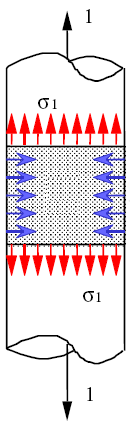
\includegraphics[scale=0.4]{ch5/image2.png}
	\captionof{figure}{Éprouvette}
\end{wrapfigure}
Soit la magnifique éprouvette représentée ci-contre. Considérons un carré loin des bords.
Supposons que l'on tire sur l'éprouvette supposée cylindrique avec deux forces opposées 
suivant l'axe $(1)$. Les flèches rouges (pleines) représentent le tenseur des contraintes
et les bleues le déplacement.\\
Selon l'axe $(1)$, il apparaît des contraintes $\sigma_1$ et des déformations $\epsilon_1$ 
liées par :
\begin{equation}
	\sigma_1 = E\epsilon_1
\end{equation}
où $E$ est le module de Young, toujours positif. Du à la symétrie de révolution, le tenseur
des contraintes n'a qu'une composante axiale ($(1)$ est une direction principale du tenseur
des contraintes, mais aussi du tenseur des déformations, par symétrie), les autres $
\tau_{ij}$ sont tous nuls : pas de contraintes de frottement.\\
    
L'expérience montre qu'en plus de la déformation $\epsilon_1$, il apparaît une contraction 
latérale proportionnelle à $\sigma_1$ (par exemple, l'iPhone 6 ! En prenant l'iPhone 5 et en
tirant dessus, on obtient quelque chose de plus fin et plus long ! Une telle innovation 
justifie bien évidemment son prix) :
\begin{equation}
	\epsilon_2 = \epsilon_3 = -\frac{\nu}{E}\sigma_1 = -\nu \epsilon_1 \leftrightarrow 
	\frac{\epsilon_2}{\epsilon_1}= -\nu\ \ \text{et }\ \ \frac{\epsilon_3}{\epsilon_1} = -\nu
\end{equation}
où $\nu$ est le coefficient de Poisson, compris entre 0 et 0,5. Quand celui-ci vaut 0,5, il
s'agit d' l'incompressibilité (le caoutchouc est déformable, mais incompressible par exemple).
Ce coefficient est très difficile à calculer en pratique.\\
    
Des "cas particuliers" sont vus dans les slides en fin de chapitre, à consulter !
